%%%%%%%%%%%%%%%%%%%%%%%%%%%%%%%%%%%%%%%%%%%%%%%%%%%%%%%%%%%%%%%%%%%%%%%%%%%%%%%%%%%%%%%%%%%%%%%%%%%%%%%%%%%%%%%%%%%%%%%%%%%%%%%%
%%%%%%%%%%%%%%%%%%%%%%%%%%%%%%%%%%%%%%%% Vorlage für Statistik-Hausarbeiten: Kopfdatei %%%%%%%%%%%%%%%%%%%%%%%%%%%%%%%%%%%%%%%%%
%%%%%%%%%%%%%%%%%%%%%%%%%%%%%%%%%%%%%%%%%%%%%%%%%%%%%%%%%%%%%%%%%%%%%%%%%%%%%%%%%%%%%%%%%%%%%%%%%%%%%%%%%%%%%%%%%%%%%%%%%%%%%%%%

%%%%%%%%%%%%%%%%%%%%%%%%%%%%%%%%%%%%%%%%%%%%%%%%%%%%%%%%%%%%%%%%%%%%%%%%%%%%%%%%%%%%%%%%%%%%%%%%%%%%%%%%%%%%%%%%%%%%%%%%%%%%%%%%
%%%%%%%%%%%%%%%%%%%%%%%%%%%%%%%%%%%%%%%%% Vorlage für Statistik-Hausarbeiten: Header %%%%%%%%%%%%%%%%%%%%%%%%%%%%%%%%%%%%%%%%%%%
%%%%%%%%%%%%%%%%%%%%%%%%%%%%%%%%%%%%%%%%%%%%%%%%%%%%%%%%%%%%%%%%%%%%%%%%%%%%%%%%%%%%%%%%%%%%%%%%%%%%%%%%%%%%%%%%%%%%%%%%%%%%%%%%


%%% Basics

\documentclass[bibtotoc, 12pt, numbers=endperiod, openbib]{scrartcl}%
\usepackage[a4paper, left=30mm, right=30mm, top=20mm, bottom=20mm, includefoot]{geometry}% Seitenränder
\usepackage[utf8]{inputenc}% in TeXnicCenter bitte umändern in: \usepackage[latin1]{inputenc}
\usepackage[T1]{fontenc}%
\usepackage[ngerman]{babel}% in englischsprachigen Arbeiten: \usepackage[english]{babel}
\usepackage{mathptmx}%
\usepackage{amsmath, amsfonts, amssymb}%
\usepackage{graphicx}%


%%%%%%%%%%%%%%%%%%%%%%%%%%%%%%%%%%%%%%%%%%%%%%%%%%%%%%%%%%%%%%%%%%%%%%%%%%%%%%%%%%%%%%%%%%%%%%%%%%%%%%%%%%%%%%%%%%%%%%%%%%%%%%%%

%%% Aussehen allgemein

\usepackage{lmodern}% Schriftart lmodern
\usepackage{setspace}% Zeilenabstand
\pagenumbering{arabic}% arabische Seitenzahlen
\setkomafont{sectioning}{\bfseries}% Serifenschrift für Überschriften
%\usepackage[small]{titlesec}%% verkleinert die Überschriften etwas
%\usepackage[singlelinecheck=0]{caption}% linksbündige Abbildungsüberschriften

\setlength{\parindent}{0em} % Keine Einrückung nach neuem Absatz

%%%%%%%%%%%%%%%%%%%%%%%%%%%%%%%%%%%%%%%%%%%%%%%%%%%%%%%%%%%%%%%%%%%%%%%%%%%%%%%%%%%%%%%%%%%%%%%%%%%%%%%%%%%%%%%%%%%%%%%%%%%%%%%%

%%% Zitate und Literaturverzeichnis

% Zitate mittels \cite[Seitenzahl]{kuerzel}
\usepackage[noadjust]{cite}%
\renewcommand\citeleft{}% Zeichen links vom Zitat, z.B. (, ggf. in die Klammer einfügen
\renewcommand\citeright{}% Zeichen rechts vom Zitat, z.B. ), ggf. in die Klammer einfügen
\renewcommand\citemid{:  }% nach der Seitenzahl folgt ": ", nach Belieben veränderbar

% Literaturverzeichnis
\makeatletter%
\renewcommand{\@biblabel}[1]{}% Literaturverzeichnis nicht nummeriert, keine Klammern um nicht vorhandene Zahlen
\makeatother%

% URLs
\usepackage[hyphens]{url}% URL im Literaturverzeichnis
\urlstyle{same}% Schriftart der URL


%%%%%%%%%%%%%%%%%%%%%%%%%%%%%%%%%%%%%%%%%%%%%%%%%%%%%%%%%%%%%%%%%%%%%%%%%%%%%%%%%%%%%%%%%%%%%%%%%%%%%%%%%%%%%%%%%%%%%%%%%%%%%%%%

%%% Häufig benötigte und nützliche Pakete

% Tabellen
\usepackage{booktabs}% Linien in Tabellen: \toprule (oben), \midrule (innerhalb der Tabelle), \bottomrule (unten)
\usepackage{longtable}% für Tabellen mit Seitenumbruch
\usepackage{ltxtable}% longtable und tabularx (Tabellen über mehrere Seiten, Gesamtbreite einstellbar)
\usepackage{dcolumn}% Tabellenspalte am Dezimaltrenner ausrichten (statt l/c/r): Format D{Dezimaltrenner in Tabelle}{Dezimaltrenner, der ausgegeben werden soll}{Dezimalstellen}

\usepackage{pdflscape}% Querformat ermöglichen
\usepackage{ziffer}% kein Abstand nach Dezimaltrenner

%%%%%%%%%%%%%%%%%%%%%%%%%%%%%%%%%%%%%%%%%%%%%%%%%%%%%%%%%%%%%%%%%%%%%%%%%%%%%%%%%%%%%%%%%%%%%%%%%%%%%%%%%%%%%%%%%%%%%%%%%%%%%%%%

\usepackage[section]{placeins} %prevent floats from being moved over it
\usepackage{flafter} %used to force floats to appear after they are defined
\usepackage{float}

\usepackage{setspace}

% Packages für Code.
\usepackage{listings}
\usepackage{xcolor}

\definecolor{codegreen}{rgb}{0,0.6,0}
\definecolor{codegray}{rgb}{0.5,0.5,0.5}
\definecolor{codepurple}{rgb}{0.58,0,0.82}
\definecolor{backcolour}{rgb}{0.95,0.95,0.92}

\lstdefinestyle{mystyle}{
    backgroundcolor=\color{backcolour},   
    commentstyle=\color{codegreen},
    keywordstyle=\color{magenta},
    %numberstyle=\tiny\color{codegray},
    stringstyle=\color{codepurple},
    basicstyle=\ttfamily\footnotesize,
    breakatwhitespace=false,         
    breaklines=true,                 
    captionpos=b,                    
    keepspaces=true,                 
    numbers=left,                    
    numbersep=5pt,                  
    showspaces=false,                
    showstringspaces=false,
    showtabs=false,                  
    tabsize=2
}

\lstset{style=mystyle}


% Theorems.
\newtheorem{example}{Beispiel}
\newtheorem{definition}{Definition}% Header, kann unverändert übernommen werden
\hyphenation{}% hier nicht korrekte Wörter eingeben: Bindestrich an Trennstellen, Wörter durch Komma getrennt (keine Umlaute)

\begin{document}%
%%%%%%%%%%%%%%%%%%%%%%%%%%%%%%%%%%%%%%%%%%%%%%%%%%%%%%%%%%%%%%%%%%%%%%%%%%%%%%%%%%%%%%%%%%%%%%%%%%%%%%%%%%%%%%%%%%%%%%%%%%%%%%%%
%%%%%%%%%%%%%%%%%%%%%%%%%%%%%%%%%%%%%%%%%%%%%%%%%%%%%%%%%%%%%%%%%%%%%%%%%%%%%%%%%%%%%%%%%%%%%%%%%%%%%%%%%%%%%%%%%%%%%%%%%%%%%%%%

%%% Titelseite
%%%%%%%%%%%%%%%%%%%%%%%%%%%%%%%%%%%%%%%%%%%%%%%%%%%%%%%%%%%%%%%%%%%%%%%%%%%%%%%%%%%%%%%%%%%%%%%%%%%%%%%%%%%%%%%%%%%%%%%%%%%%%%%%
%%%%%%%%%%%%%%%%%%%%%%%%%%%%%%%%%%%%%%%% Vorlage für Statistik-Hausarbeiten: Titelseite %%%%%%%%%%%%%%%%%%%%%%%%%%%%%%%%%%%%%%%%
%%%%%%%%%%%%%%%%%%%%%%%%%%%%%%%%%%%%%%%%%%%%%%%%%%%%%%%%%%%%%%%%%%%%%%%%%%%%%%%%%%%%%%%%%%%%%%%%%%%%%%%%%%%%%%%%%%%%%%%%%%%%%%%%


\thispagestyle{empty}%

{\raggedright%
Otto-Friedrich-Universität Bamberg\\% ggf. Namen der Universität eintragen
Lehrstuhl für Statistik und Ökonometrie\\%
Standort: Bamberg\\% eigenen Standort auswählen
Sommersemester 2022\\% Winter-/Sommersemester eintragen
Vorlesung: Blockseminar Survey-Methodik\\% Titel der Veranstaltung eintragen
Prüfer: Dr. Sara Bleniger\\% Name eintragen
}%

\vspace*{\fill}%
\begin{center}%
    \textbf{\Huge{Statistische Geheimhaltung:}}%
\end{center}%
\begin{center}%
    {\linespread{2.5}
    \textbf{\Huge{Cell Key Methode}}%
    }
\end{center}%
\vfill%

{\vspace*{\stretch{1}}%
\raggedleft%
Joshua Simon\\% eintragen
joshua-guenter.simon@stud.uni-bamberg.de\\% eintragen
Master Survey Statistik, 4. Fachsemester\\% eintragen
Matrikelnummer: 2032411\\%
\today\\}% fügt das aktuelle Datum ein, ggf. manuell ändern


\newpage%

%%%%%%%%%%%%%%%%%%%%%%%%%%%%%%%%%%%%%%%%%%%%%%%%%%%%%%%%%%%%%%%%%%%%%%%%%%%%%%%%%%%%%%%%%%%%%%%%%%%%%%%%%%%%%%%%%%%%%%%%%%%%%%%%% Angaben im Dokument ändern


%%%%%%%%%%%%%%%%%%%%%%%%%%%%%%%%%%%%%%%%%%%%%%%%%%%%%%%%%%%%%%%%%%%%%%%%%%%%%%%%%%%%%%%%%%%%%%%%%%%%%%%%%%%%%%%%%%%%%%%%%%%%%%%%

%%% Verzeichnisse

\tableofcontents% Inhaltsverzeichnis
\newpage%

\listoffigures% Abbildungsverzeichnis
\listoftables% Tabellenverzeichnis
\lstlistoflistings

\newpage%
%%%%%%%%%%%%%%%%%%%%%%%%%%%%%%%%%%%%%%%%%%%%%%%%%%%%%%%%%%%%%%%%%%%%%%%%%%%%%%%%%%%%%%%%%%%%%%%%%%%%%%%%%%%%%%%%%%%%%%%%%%%%%%%%

%%% Darstellender Teil

\onehalfspacing% Zeilenabstand


\section{Einführung}%

Die amtliche Statistik sorgt mit einer Vielzahl an Veröffentlichungen für die Bereitstellung von aufbereiteten statistischen Informationen. Damit geht sie dem Ziel nach, Bürgern, Institutionen und anderen gesellschaftlichen Einrichtungen eine Datengrundlage für die Entscheidungsfindung zu bieten. Weiter dient die amtliche Statistik auch der Politik und der Wissenschaft als Datenquelle. Das Sammeln und Erheben dieser Daten stellt in vielen Fällen einen Eingriff auf das Recht der informationellen Selbstbestimmung für Personen und Entitäten dar. Dieses Recht ist das Fundament des mordernen Datenschutzes und wird über Artikel 2 des Grundgesetztes abgedeckt. Es steht au\ss er Frage, dass dieses Recht besonders schützenswert ist. Demnach steht auch die amtliche Statistik in der Pflicht dieser Verantwortung nachzukommen. Konkret manifestiert sich das Einhalten dieser Plficht in dem sog. Statistikgeheimnis. Aus dem Bundestatistikgesetzt lässt sich hierzu der folgende Absatz aufgreifen (\S 16 Abs. 1 Satz 1 BStatG):

\textit{\glqq Einzelangaben über persönliche und sachliche Verhältnisse, die für eine Bundesstatistik gemacht werden, sind von den Amtsträgern und für den öffentlichen Dienst besonders Verpflichteten, die mit der Durchführung von Bundesstatistiken betraut sind, geheim zu halten, soweit durch besondere Rechtsvorschrift nichts anderes bestimmt ist.\grqq{}}

Konkret möchte man mit der statistischen Geheimhaltung einen Schutz für einzelne Person und Entitäten vor der Offenlegung ihrer sensitven Daten bieten. Dies dient im Weiteren auch der Aufrechterhaltung des Vertrauensverhältnisses zwischen den Befragten und den statistischen Ämtern und erhebenden Einrichtungen. Dies gewährleistet abermals die Zuverlässigkeit der Angaben und der Berichtswilligkeit der Befragten. Die vorausgegangenen Punkte werden in einer Begrüdung zum BStatG erwähnt [\cite{Nickl}]. Ausnahmen von einer Geheimhaltung bestehen nur in Ausnahmefällen, z.B. wenn eine explizite Einwillung zur Veröffentlichung durch den Befragten vorliegt oder wenn sich die Informationen aus allgemein zugänglichen Quellen von öffentlichen Stellen beziehen. Auch die inner-beördliche Übermittlung, Methodenentwicklung, Planungs- und Forschungszwecke werden über das BStatG geregelt.

Im weiteren Verlauf dieser Arbeit sollen Geheimhaltungsverfahren und Geheimhaltungsregeln präsentiert werden, die im Einzelnen die statistische Geheimhaltung gewährleisten und damit dem Statistikgeheimnis der amtlichen Statistik nachkommen. Besondere Beachtung wird dabei der Cell Key Methode (CKM) geschenkt. Dieses Verfahren bietet ein Ansatz, welcher gegenüber anderen Verfahren gut zu Implementieren und zu Automatisieren ist. Gerade dieser Punkt ist in einem immer weiter werdenden technolgischen Umfeld nicht au\ss er Acht zu lassen.

%%%%%%%%%%%%%%%%%%%%%%%%%%%%%%%%%%%%%%%%%%%%%%%%%%%%%%%%%%%%%%%%%%%%%%%%%%%%%%%%%%%%%%%%%%%%%%%%%%%%%%%%%%%%%%%%%%%%%%%%%%%%%%%%%%%%%%%%%%%%

%\newpage
\section{Etablierte Geheimhaltungsverfahren}

In diesem Abschnitt sollen zunächst die grundlegenden Begrifflichkeiten für Geheimhaltungsverfahren und Geheimhaltungsregeln beschrieben werden. 

\subsection{Methodische Grundlagen}

Grundsätzlich gibt es zwei sich unterscheidenede methodische Ansätze, die bei der Geheimhaltung zum Tragen kommen können. Zum einen existieren \textit{informationsreduzierende Methoden}. In der Gattung dieser Verfahren werden durch Aggregation oder Sperrrung kritische Kategorien oder Werte die Aufdeckungsrisiken verhindert. Eine Aggregation meint in diesem Fall das Zusammenfassen zu übergeordneteten Positionen, z.B. durch Summation kleinerer Positionen. Bei einer Sperrung ist auch oft von einer Löschung die Rede. Hier werden gezielt einzelne Werte identifiziert und aus der Tabelle entfernt. Als Kontrast stehen \textit{datenverändernde Methoden} gegenüber. Hier werden durch gezielte Veränderungen der Daten - beispielsweise durch Runden oder Zufallsüberlagerungen - kritische Werte verfälscht, was auch für eine erfolgreiche statistische Geheimhaltung sorgen kann. 

Weiter differenziert man Geheimhaltungsverfahren auch nach dem Zeitpunkt ihrer Durchführung. Die Daten können bereits vor der Tabellierung mit einer Geheimhaltung versehen werden. Man spricht hier von \textit{pre-tabulare Verfahren}. Diese Verfahren werden als Anonymisierung bezeichnet, da die Daten im Vorfeld so verändert werden, dass keine kritischen Ergebnisse resultieren. Oftmals ist diese Art von Geheimhaltung aber nicht ausreichend, weshalb weitere Verfahren im Anschluss angewandt werden müssen. Man spricht nun von \textit{post-tabulare Verfahren}. Ihre Mechanismen werden auf die ferig tabellierten Daten angewandt.


\subsection{Statistische Tabellen}

Gegenstand der Geheimhaltung stellen in dieser Arbeit statistische Tabellen dar. Ein Gro\ss teil der Veröffentlichungen der amtlichen Statistik sind selbst - oder beinhalten - statistische Tabellen, welche aus den amtlichen Daten abgeleitet werden. Ma\ss gebend für die Anwendung eines Geheimhaltungsverfahrens ist die Art der zu veröffentlichenden Tabelle, die vorliegt. Man unterscheidet im allgemeinen zwischen \textit{Häufigkeitstabllen} und \textit{Wertetabellen}. Erstere stellen Häufigkeiten oder Fallzahlen dar, z.B. die Anzahl von Frauen und Männern innerhalb einer Universitätät. Wertetabellen hingegen stellen Wertesummen wie Umsätze dar. Diese unterschiedlichen Kontexte, in denen die Zahlen dieser Tabellen interpretiert werden können, fordern eine natürliche Unterscheidung innerhalb der Geheimhaltung. Es folgen zwei einfache Beispiel für diese Tabellentypen mit rein fiktiven Ausprägungen.

\begin{table}[h]
    \centering
    \begin{tabular}{ r r r r }
        \textbf{Studienfach} \vline & \textbf{männlich} & \textbf{weiblich} & \textbf{insgesamt} \\ 
        \hline
        Bauingenieurwesen \vline & $4$ & $3$ & $7$ \\
        Informatik \vline & $9$ & $12$ & $21$ \\  
        Medizin \vline & $4$ & $1$ & $5$ \\
        Survey Statistik \vline & $10$ & $10$ & $20$ \\
        \hline
        Gesamt \vline & $27$ & $26$ & $53$
    \end{tabular}
    \caption{Beispiel für eine Häufigkeitstabelle}
\end{table}

\begin{table}[h]
    \centering
    \begin{tabular}{ r r r r r }
        \textbf{Brauerei} \vline & \textbf{Mährs Bräu} & \textbf{Schinkerla} & \textbf{Käsmann} & \textbf{Gesamt} \\ 
        \hline
        Umsatz \vline & $600.000$ & $50.000$ & $250.000$ & $900.000$
        \end{tabular}
    \caption{Beispiel für eine Wertetabelle}
\end{table}


\subsection{Bewährte Ansätze}


%%%%%%%%%%%%%%%%%%%%%%%%%%%%%%%%%%%%%%%%%%%%%%%%%%%%%%%%%%%%%%%%%%%%%%%%%%%%%%%%%%%%%%%%%%%%%%%%%%%%%%%%%%%%%%%%%%%%%%%%%%%%%%%%%%%%%%%%%%%%


\section{Cell Key Methode}

Die im vorherigen Kapitel beschrieben Geheimhaltungsverfahren müssen in der Regel - zumindest bis zu einem gewissen Grad - manuell durchgeführt werden und eine Automatisierung ist eher unfelxibel. Mit der \textit{Cell Key Methode (CKM)} wird ein Geheimhaltungsverfahren präsentiert, welches gut zu automatisieren und vergleichsweise einfach zu implementieren ist. Die Cell Key Methode ist auch als \textit{ABS-Verfahren} bekannt. Der Name stammt von der schöpfenden Institutuion des Verfahrens, dem Australian Bureau of Statistics, ab. Durch die Verwendung von zufallsbasierten Additionen, den sog. Überlagerungen, werden Datenwerte verschleiert. Der Ermittlung einer solchen zufallsbasierten Addition liegt eine einmalig festzulegende Wahrscheinlichkeitsverteilung mit den möglichen Überlagerungswerten zugrunde [\cite{Enderle}]. Für die Bestimmung dieser Überlagerungen wird ein deterministischer Mechaniusmus eingesetzt. Dieser nutzt den original Zellwert und den sog. Cell-Key um aus der Verteilung der Überlagerungswerte eine eindeutige Überlagerung zu ziehen [\cite{Enderle}]. Eine mit dem CKM Verfahren geheimgehaltene Tabelle veröffentlicht also die Summe aus Originalwerten und Überlagerungen. Die CKM zählt damit zu den datenveränderndeden Verfahren.

\subsection{Verfahrensparamter und Überlagerungsmatrix}

An statistische Geheimhaltungsverfahren, insbesondere den datenverändernden Verfahren, werde bestimmte Anforderungen gestellt. Für die Cell Key Methode werden in der amtlichen Statistik gewisse stochastische Eigenschfaten gefordert, um die Qualität und Nachvollziehbarkeit der Ergebnisse zu sichern. Zu diesen Eigenschaften zählt einerseits die Unverzerrtheit der Überlagerungen [\cite{Enderle}]. Damit meint man, dass der Überlagerungswert, welcher zu den Originalwerten addiert wird, im Mittel gleich Null ist. Es soll also die Erwartungstreue $E(z) = 0$ gelten. Darüber hinaus fodert man ebenfalls eine konstante Streuung der Verteilung der Überlagerungen [\cite{Enderle}]. Es soll die Varianz erhalten bleiben, also $Var(z) = s^2$ gelten. Um diese beiden Eigenschaften zu kokretisieren, werden Verfahrensparamter eingeführt. Diese dienen weiter auch dazu das Geheimhaltungsverfahren - und damit die Überlagerungen - an verschiedene Kontexte anzupassen. Zu diesen Verfahrensparamter zählen nach [\cite{Höhne}]:

\begin{itemize}
    \item Eine boolsche Variable, die angibt, ob Originalwerte $1$ und $2$ geheimgehalten werden sollen.
    \item Der Anteil $p_0$ der nicht zu überlagernden Originalwerte.
    \item Die Maximalüberlagerung $d$.
    \item Die Standardabweichung der Überlagerungsbeiträge $s$.
\end{itemize}

Gestand des Interesses sind demnach Zufallsfunktionen $z$, die eine bedingte Wahrscheinlichkeitsverteilung auf die Originalwerte $i$ mit Zielhäufigkeit $j$ darstellen. Man sucht also für jeden Originalwert $i = \{0, 1, 2, \dots, n \}$ eine Wahrscheinlichkeitsverteilung der Form $z = p_i$ mit den Wahrscheinlichkeiten für die Übergänge $v_i$ hin zu den Zielhäufigkeiten $j$ [\cite{Enderle}]. Diese Wahrscheinlichkeiten bilden ein nicht-lineares Gleichungssystem, in welchem die zuvor genannten stochastischen Eigenschaften als Nebenbedinungen eingehen. Diese lassen sich nun als 

\begin{align}
    E(z) & = \sum_{i = -d}^{d} p_i v_i = 0 \\
    Var(z) & = \sum_{i = -d}^{d} p_i v_{i}^{2} = s^2 \\
    & \sum_{i = -d}^{d} p_i = 1
\end{align}

schreiben [\cite{Höhne}]. Dabei wird in der letzten Zeile $(3)$ noch gefordert, dass die Summe der Übergangswahrscheinlichkeiten für einen Originalwert gleich $1$ ist. Die Lösung dieses Problems lässt sich in Matrixform notieren. Man spricht hier von der sog. Überlagerungsmatrix mit Zeilen $i$ und Spalten $j$, welche zur Bestimmung der Überlagerungsbeiträge $j$ zu den Originalwerten $i$ verwendet werden kann. Für weitere mathematische Details und Lösungsansätze sei an dieser Stelle auf [\cite{Giessing}] verwiesen. In [\cite{Höhne}] wird die Lösung eines solchen Gleichungssystems für die Verfahrensparamter $p_0 = 0,5 = 50\%$, $d = 4$ und $s = 2,25$ gezeigt. Diese Überlagerungsmatrix ist in Abbildung \ref{matrix_plot} in Form einer Heatmap zu sehen. Der \textit{Python} Code zum Erstellen dieser Grafik ist in Anhang A zu finden.

\begin{figure}[H]
    \begin{center}
        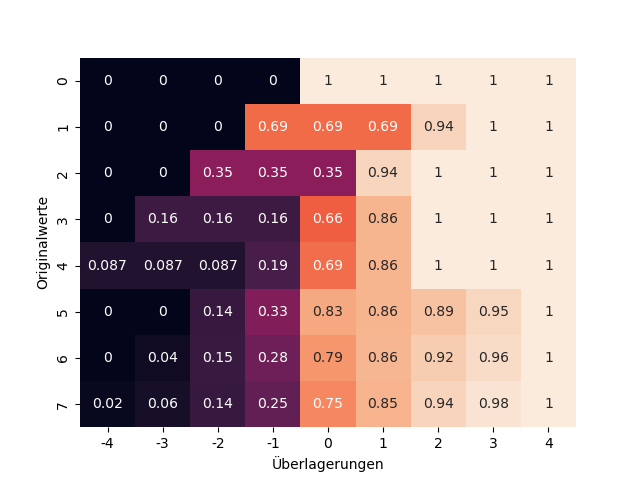
\includegraphics[width=0.85\textwidth]{img/matrix.png}
        \caption{Beispiel für eine Überlagerungsmatrix mit Übergangswahrscheinlichkeiten für paarige Originalwerte und Zielhäufigkeiten}
        \label{matrix_plot}
    \end{center}
\end{figure}

Es ist hierbei anzumerken, dass direkt eine symmetrische Verteilung für die Überlagerungsbeiträge gewählt wurde. Auf der $x$-Achse sind die anzuwendenden Überlagerungswerte von $-d$ bis $d$ zu sehen. Auf der $y$-Achse sind die Originalwerte abgetragen. In der jeweiligen Zelle sind die einzelnen Übergangswahrscheinlichkeiten abzulesen. Für Originalwerte  grö\ss er $7$ ist die Zeile für Originalwerte gleich $7$ ma\ss gebend. Die Überlagerungsmatrix bildet den Kern der CKM. Ihre Anwendung wird im nächsten Abschnitt beschrieben.


\subsection{Methodik und Verfahrensdurchführung}%

Die wichtigsten Bestandteile des Verfahrens werden in [\cite{Enderle}] dargestellt. Ähnlich wie in [\cite{Wipke}] beschrieben, lässt sich nun ein Algorithmus formulieren. Ausgangspunkt sind die in einer Statistik erhobenen Mikrodaten bzw. Mikrodatensätze. Das sind die plausibilisierten Einzeldatensätze. 

\begin{enumerate}
    \item Erzeugung der Originalwerte mit einem Auswertungstool
    \item Cell-Key-Bestimmung aus Zufallszahlen innerhalb des Auswertungs-Tools
    \item Lookup-Modul
    \begin{enumerate}
        \item Auslesen der Überlagerungswerte aus der Überlagerungsmatrix
        \item Addieren der Überlagerungswerte und Originalwerte
    \end{enumerate}
\end{enumerate}

Die folgende Abbildung \ref{fig_ckm_chart} visualisiert den schehmatischen Ablauf des zuvor beschrieben Algorithmus. Im Wesentlichen werden zwei technische System benötigt, um das Verfahren zu realisieren. Zum einen wird ein Auswertungstool benötigt, welches die gespeicherten Mikrodaten in Tabellenform bringt. Mit Hilfe des Lookup-Moduls werden dann die beiden Eingangsgrö\ss en - Originalwerte und Cell-Keys - verwendet, um die Überlagerungswerte aus der Überlagerungsmatrix zu bestimmen. Diese Überlagerungswerte werden letztlich auf die Originalwerte addiert und stellen damit die finalen Werte für die Veröffentlichung dar. 

\begin{figure}[H]
    \begin{center}
        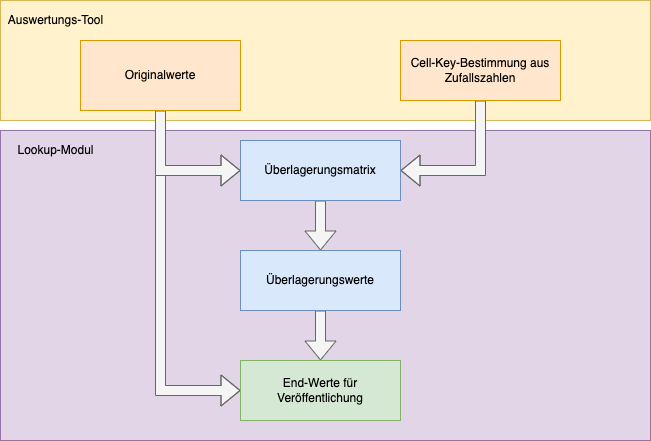
\includegraphics[width=0.85\textwidth]{img/ckm_flow.png}
        \caption{Ablaufdiagramm der Cell Key Methode}
        \label{fig_ckm_chart}
    \end{center}
\end{figure}

Die Einzelschritte des Verfahrens sollen nun im Detail beleuchtet werden.

\subsubsection{Erzeugung der Originalwerte}

Dieser Schritt ist spezifisch für die jeweilige Zieltablle, die veröffentlicht werden soll. Im Allgemeinen werden Filterungen anhand bestimmter Merkamle vorgenommen und dann Summen der Fallzahlen gebildet. Für diese Operation - also die Tabellierung - führt man die Beizeichnung $f$ ein.

\subsubsection{Cell-Key-Bestimmung}

Für die Bestimmung des Cell-Keys wird jedem Mikrodatensatz zunächst eine gleichverteile Zufallszahl $r$, der sog. \textit{Record-Key}, mit $r \sim \mathcal{U}(0, 1)$ zugeordnet. Mit diesen Record-Keys wird dieselbe Auswertungstabelle wie mit den Originalwerten gebildet. Man führt also diesseble  Operation $f$ auf den Daten durch, wie in Abschnitt 3.1.1. Es ergeben sich also Summen von Record-Keys. Von diesen Record-Key Summen werden nur die Nachkommastellen betrachtet. Dieser Wert definiert den \textit{Cell-Key} [\cite{Enderle}]. Um dieses Vorgehen zu verdeutlichen soll das folgende Beispiel aus der Hochschulstatistik betrachtet werden. Tabelle \ref{tab_mikrodaten} zeigt die Mikrodaten mit Record-Keys, wie sie in einer Datenbank gespeichert sein könnten.

\begin{table}[h]
    \centering
    \begin{tabular}{ r r r r }
        \textbf{ID} \vline & \textbf{Universitätät} & \textbf{Geschlecht} & \textbf{Record-Key} \\ 
        \hline
        $1$ \vline & Würzburg & m & $0,611853$ \\
        $2$ \vline & Eichstätt & w & $0,139494$ \\
        $3$ \vline & München & w & $0,292145$ \\
        $4$ \vline & München & m & $0,366362$ \\
        $5$ \vline & Würzburg & m & $0,456070$ \\
        $6$ \vline & Würzburg & m & $0,785176$ \\
        $7$ \vline & Bamberg & m & $0,199674$ \\
        $8$ \vline & München & w & $0,514234$ \\
        $9$ \vline & München & m & $0,592415$ \\
        $10$ \vline & München & m & $0,046450$
    \end{tabular}
    \caption{Mikrodaten mit Record-Keys}
    \label{tab_mikrodaten}
\end{table}

Tabelle \ref{tab_agg} stellt die Daten nach Durchführung der Tabellierung $f$ dar. Die Daten wurden hier nach der Universitätät und nach dem Geschlecht zusammengefasst. Die entsprechenden Fallzahlen, Record-Key-Summen und Cell-Keys werden abgebildet. 

\begin{table}[h]
    \centering
    \begin{tabular}{ r r r r r r}
        \textbf{ID} \vline & \textbf{Universitätät} & \textbf{Geschl.} & \textbf{Fallzahl} & \textbf{Record-Key-Summe} & \textbf{Cell-Key} \\ 
        \hline
        $1$ \vline & Bamberg & m & $1$ & $0,199674$ & $0,199674$ \\
        $2$ \vline & Eichstätt & w & $1$ & $0,139494$ & $0,139494$ \\
        $3$ \vline & München & m & $3$ & $1,005227$ & $0,005227$ \\
        $4$ \vline & München & w & $2$ & $0,806379$ & $0,806379$ \\
        $5$ \vline & Würzburg & m & $3$ & $1,853099$ & $0,853099$
    \end{tabular}
    \caption{Aggregierte Daten mit Record-Key-Summen und Cell-Key}
    \label{tab_agg}
\end{table}

Die Werte in Zeile 5 von Tablle \ref{tab_agg} ergeben sich durch Zählen der Zeilen in Tabelle \ref{tab_mikrodaten}, in denen $Universität\ddot{a}t = W\ddot{u}rzburg \: \wedge \: Geschlecht = m$. Die Record-Key-Summe in dieser Zeile ergibt sich nach $0,611853 + 0,456070 + 0,785176 = 1,853099$. Der daraus abgeleitete Cell-Key beträgt damit $0,853099$.

\subsubsection{Lookup-Modul}

Im Anschluss an die Bestimmung der Originalwerte und der dazugehörigen Cell-Keys gilt es nun die Überlagerungen zu berechnen. Für die Bestimmung eines Überlagerungswertes dient das Paar $(Originalwert, \; CellKey)$ als Input. Damit meint man den Wert einer einzelnen Tabellenzelle und den über dieselbe Operation $f$ berechneteten Cell-Key. Das Lookup Modul stellt die Funktionalität bereit, anhand dieses Wertepaares den zugehörigen Überlagerungswert aus der Überlagerungsmatrix abzulesen. Um dies weiter zu illustrieren wird die Überlagerungsmatrix aus Abbildung \ref{matrix_plot} herangezogen. Betrachtet man Zeile 5 aus Tabelle \ref{tab_agg}, so liegt das Paar $(Originalwert = 3, \; CellKey = 0,853099)$ vor. Um nun auch den dazu passenden Überlagerungswert zu bestimmen, wählt man die Zeile $i$ der Überlagerungsmatrix, die dem $Originalwert$ - hier also $3$ - entspricht. Anschlie\ss end bestimmt man mit Hilfe des $CellKey$ die Spalte $j$, für welche der Wert in der Matirx erstmalig kleiner als $CellKey$ ist. In diesem Fall führt dies zu $j = 1$, da $0,853099 < 0.86$. Der Wert $j = 1$ ist damit der zu addierende Überlagerungswert. Daraus ergibt sich ein finaler Wert von $3 + 1 = 4$. Wendet man dieses Vorgehen vollständig auf das Beispiel aus Tabelle \ref{tab_agg} an, so ergeben sich die finalen und damit geheimgehaltenen Werte aus Tabelle \ref{tab_final}.

\begin{table}[h]
    \centering
    \begin{tabular}{ r r r r r r}
        \textbf{ID} \vline & \textbf{Universitätät} & \textbf{Geschl.} & \textbf{Fallzahl} & \textbf{Überlagerung} & \textbf{Finaler Wert} \\ 
        \hline
        $1$ \vline & Bamberg & m & $1$ & $-1$ & $0$ \\
        $2$ \vline & Eichstätt & w & $1$ & $-1$ & $0$ \\
        $3$ \vline & München & m & $3$ & $-3$ & $0$ \\
        $4$ \vline & München & w & $2$ & $1$ & $3$ \\
        $5$ \vline & Würzburg & m & $3$ & $1$ & $4$
    \end{tabular}
    \caption{Überlagerungen und final geheimgehaltene Werte}
    \label{tab_final}
\end{table}

In Anhang A ist eine \textit{Python} Realisierung dieses Verfahrens zu finden.


\subsection{Besonderheiten der Cell Key Methode}%

Eine Besonderheit, die sich aus der Verwendung der Cell Key Methode ergibt, ist die Nicht-Additivität des Verfahrens. Dadruch, dass Rand- und Zwischensummen nicht erst nach der Geheimhaltung, sondern ebenfalls während der Tabellierung gebildet werden, unterliegen auch diese Werte dem Geheimhaltungsmechanismus. Um dies zu veranschaulichen soll abschlie\ss end ein weiteres Fallbeispiel aus der Hochschulstatistik betrachtet werden. Tabelle \ref{tab_additivity} zeigt für eine Universitätät jeweils eine Insgesamt-Position \textit{i} sowie die Unterteilung nach dem Geschlecht \textit{m} und \textit{w}. Es sind sowohl die Originalwerte als auch die final überlagerten Werte abgebildet. Auch die Positionen für die Zwischensummen \textit{i} wurden mit der Tabellierungs-Operation $f$ auf Basis der Originalwerte und der Record-Keys gebildet. Damit entsteht also ein eigner Cell-Key und Überlagerungswert für diese Zahlen. Für das Beispiel der Universität Bamberg aus Tabelle \ref{tab_additivity} sieht man schnell, dass für die Originalwerte die gewohnte Additivität vorhanden ist, denn $166 = 75 + 91$. Führt man diese Betrachtung allerdings auf den überlagerten Werten durch, so erhält man eine falsche Aussage, denn $168 \neq 75 + 91$. Diese Phänomen bezeichnet man als \textit{Nicht-Additivität} einer statistischen Tabelle.

\begin{table}[h]
    \centering
    \begin{tabular}{ r r r r r}
        \textbf{ID} \vline & \textbf{Universitätät} & \textbf{Geschl.} & \textbf{orig. Fallzahl} & \textbf{überl. Fallzahl} \\ 
        \hline
        $1$ \vline & Bamberg & i & $166$ & $168$ \\
        $2$ \vline & Bamberg & m & $75$ & $75$ \\
        $3$ \vline & Bamberg & w & $91$ & $91$ \\
        $4$ \vline & Eichstätt & i & $46$ & $48$ \\
        $5$ \vline & Eichstätt & m & $17$ & $20$ \\
        $6$ \vline & Eichstätt & w & $32$ & $29$
    \end{tabular}
    \caption{Beispiel zur Nicht-Additivität der CKM}
    \label{tab_additivity}
\end{table}

Diese Nicht-Additivität wird beim Cell Key Verfahren in Kauf genommen, da im Weiteren zwei konkrete Vorteile dieser Methode überwiegen. Das unabhängige und separate Überlagern von Tabellenfeldern führt zu zwei wichtigen Vorteilen dieses Geheimhaltungsverfahrens [\cite{Enderle}]. Zum einen wird eine \textit{tabellenübergreifenede Konsistenz} erreicht. Die zu addierenden Überlagerungswerte zu einem bestimmten Originalwert (z.B. Studierende der Universitätät Bamberg) sind bei gleicher Datengrundlage immer identisch - unabhängig von der Zieltabelle. Dies ergibt sich aus den einmalig zugespielten Record-Keys und dem danach folgenden deterministeischen Lookup-Modul. Der zweite überwiegende Vorteil der CKM ist die \textit{Genauigkeit} des Verfahrens [\cite{Enderle}]. Dieser Punkt beschreibt die Vermeidung von zufällig gleichgerichteten Überlagerungen. Dies würde im Einzelfall zu grö\ss eren Veränderungen zwischen Original- und geheimgehaltenen Wert führen. Durch die Überlagerung aller Tabellenzellen umgeht man diese Gefahr.

\subsection{Aufdeckungsrisiko}



%%%%%%%%%%%%%%%%%%%%%%%%%%%%%%%%%%%%%%%%%%%%%%%%%%%%%%%%%%%%%%%%%%%%%%%%%%%%%%%%%%%%%%%%%%%%%%%%%%%%%%%%%%%%%%%%%%%%%%%%%%%%%%%%%%%%%%%%%%%%

%\newpage
\section{Zusammenfassung und Fazit}

Damit das Bayerische Landesamt für Statistik seiner gesetzlich vorgeschrieben Pflichten nachkommen kann, sind die unterschiedlichsten Technologien und Verfahren notwendig. Neben dem Erheben der Daten bei den Meldern, gehören auch die Plausibilisierung und die Aufbereitung der Daten zu seinen Aufgaben. Um eine so große Datenmenge effizient zu verarbeiten, wird auf moderne Lösungen aus der Informationstechnologie zurückgriffen. Hierzu zählen verschiedene Skriptsprachen, Datenbanken und Datawarehouses. Um die Qualität der Daten zu wahren, sind neben rein technischer Kontrollen auch sehr fachliche Zusammenhänge zu prüfen und ggf. zu korrigieren. Dies erfordert ein tiefes inhaltliches Verständnis der Daten und ihrer Merkmale. Eine gewisse Interpretation und Analyse sind also auch im Data Engineering notwendig, um die Datenqualität und den Datenfluss zu erhalten, sowie die Daten zu publizieren und damit die Pflicht der amtlichen Statistik zu erfüllen. 

\newpage%
%%%%%%%%%%%%%%%%%%%%%%%%%%%%%%%%%%%%%%%%%%%%%%%%%%%%%%%%%%%%%%%%%%%%%%%%%%%%%%%%%%%%%%%%%%%%%%%%%%%%%%%%%%%%%%%%%%%%%%%%%%%%%%%%
%%%%%%%%%%%%%%%%%%%%%%%%%%%%%%%%%%%%%%%%%%%%%%%%%%%%%%%%%%%%%%%%%%%%%%%%%%%%%%%%%%%%%%%%%%%%%%%%%%%%%%%%%%%%%%%%%%%%%%%%%%%%%%%%

%%% Literaturverzeichnis
%%%%%%%%%%%%%%%%%%%%%%%%%%%%%%%%%%%%%%%%%%%%%%%%%%%%%%%%%%%%%%%%%%%%%%%%%%%%%%%%%%%%%%%%%%%%%%%%%%%%%%%%%%%%%%%%%%%%%%%%%%%%%%%%
%%%%%%%%%%%%%%%%%%%%%%%%%%%%%%%%%% Vorlage für Statistik-Hausarbeiten: Literaturverzeichnis %%%%%%%%%%%%%%%%%%%%%%%%%%%%%%%%%%%%
%%%%%%%%%%%%%%%%%%%%%%%%%%%%%%%%%%%%%%%%%%%%%%%%%%%%%%%%%%%%%%%%%%%%%%%%%%%%%%%%%%%%%%%%%%%%%%%%%%%%%%%%%%%%%%%%%%%%%%%%%%%%%%%%


\begin{thebibliography}{9}
    % beliebige Zahl steht für die Anzahl der Quellen, z.B. 10 Quellen - zweistellige Zahl, 69 Quellen - zweistellige Zahl, 157 Quellen - dreistellige Zahl
\singlespacing%

\bibitem[Enderle, 2019]{Enderle} 
Enderle, Tobias und Meike Vollmar: Geheimhaltung in der Hochschulstatistik. \emph{WISTA} | 6, Statistisches Bundesamt (Destatis), Wiesbaden 2019.

\bibitem[Giessing, 2016]{Giessing} 
Giessing, Sarah: Computational Issues in the Design of Transition Probabilities and Disclosure Risk Estimation for Additive Noise.
\emph{LNCS}, vol. 9867, Springer International Publishing, 2016.

\bibitem[Höhne, 2019]{Höhne} 
Höhne, Jörg und Julia Höninger: Die Cell-Key-Methode – ein Geheimhaltungsverfahren. \emph{Statistische Monatshefte Niedersachsen} 1, 2019.

\bibitem[Nickl, 2019]{Nickl} 
Nickl, Andreas: Datenschutz, Geheimhaltung, Anonymisierung. \emph{Einfuührungsfortbildung} Bayerisches Landesamt für Statistik, Fürth, 2019.

\bibitem[Rothe, 2015-5]{Rothe-1} 
Rothe, Patrick: Statistische Geheimhaltung – Der Schutz vertraulicher Daten in der amtlichen Statistik - Teil 1: Rechtliche und methodische Grundlagen \emph{Bayern in Zahlen} 5, Bayerisches Landesamt für Statistik, München, 2015.

\bibitem[Rothe, 2015-8]{Rothe-2} 
Rothe, Patrick: Statistische Geheimhaltung – Der Schutz vertraulicher Daten in der amtlichen Statistik - Teil 2: Herausforderungen und aktuelle Entwicklungen. \emph{Bayern in Zahlen} 8, Bayerisches Landesamt für Statistik, München, 2015.

\bibitem[Wipke, 2018]{Wipke} 
Wipke, Mirko: Geheimhaltung im Data Warehouse - Prototypische Implementierung von automatisierter Geheimhaltung im Data Warehouse für die amtliche Hochschulstatistik in Bayern. \emph{Bayern in Zahlen} 12, Bayerisches Landesamt für Statistik, Fürth, 2018.


%\bibitem[Name, wie er mit cite im Text zitiert wird]{kuerzel ohne Umlaute, das mit cite angesprochen wird}%
%Nachname, Vorname (Jahr): \emph{Buchtitel}. Ort: Verlag.%

%\bibitem[Autor 2013]{mimimi}%
%Nachname, Vorname (Jahr): Artikel, in: \emph{Zeitschrift} Auflage, S. XX-YY.%

%\bibitem[Autor et\,al. 1999]{magnicht}%
%Nachname, Vorname (o.\,J.): Titel, online verfügbar unter: \url{http...} (Zugriff am \today).%

\end{thebibliography}%

\newpage%

%%%%%%%%%%%%%%%%%%%%%%%%%%%%%%%%%%%%%%%%%%%%%%%%%%%%%%%%%%%%%%%%%%%%%%%%%%%%%%%%%%%%%%%%%%%%%%%%%%%%%%%%%%%%%%%%%%%%%%%%%%%%%%%%%

\newpage 
\appendix
\section{Python Implementierung}

Nachfolgend ist die vollständige \textit{Python} Implementierung des CKM Verfahrens für ein Testbeispiel aus der Hochschulstatistik abgebildet.

\lstinputlisting[language=Python, caption=CKM Python Beispiel]{../src/ckm.py}

%%%%%%%%%%%%%%%%%%%%%%%%%%%%%%%%%%%%%%%%%%%%%%%%%%%%%%%%%%%%%%%%%%%%%%%%%%%%%%%%%%%%%%%%%%%%%%%%%%%%%%%%%%%%%%%%%%%%%%%%%%%%%%%%
%%%%%%%%%%%%%%%%%%%%%%%%%%%%%%%%%%%%%%%%%%%%%%%%%%%%%%%%%%%%%%%%%%%%%%%%%%%%%%%%%%%%%%%%%%%%%%%%%%%%%%%%%%%%%%%%%%%%%%%%%%%%%%%%

%%% Wahrheitsgemäße Erklärung

\newpage 
\noindent%
Ich erkläre hiermit, dass ich die Seminararbeit mit dem Titel \emph{Statistische Geheimhaltung: Cell Key Methode} im \emph{Sommersemester 2022} selbständig angefertigt, keine anderen Hilfsmittel als die im Literaturverzeichnis genannten benutzt und alle aus den Quellen und der Literatur wörtlich oder sinngemä\ss übernommenen Stellen als solche gekennzeichnet habe.%
\bigskip
 
\noindent%
\emph{Bamberg}, den \today\\%
\emph{Unterschrift}%

\end{document}%

%%%%%%%%%%%%%%%%%%%%%%%%%%%%%%%%%%%%%%%%%%%%%%%%%%%%%%%%%%%%%%%%%%%%%%%%%%%%%%%%%%%%%%%%%%%%%%%%%%%%%%%%%%%%%%%%%%%%%%%%%%%%%%%%